\documentclass[11pt]{article}
\usepackage{amsthm}
\usepackage{amsmath}
\usepackage{amssymb}
\usepackage[spanish,es-tabla]{babel}
\usepackage[style=numeric,sorting=none]{biblatex}
\usepackage{bm}
\usepackage{booktabs}
\usepackage{enumitem}
\usepackage{fancyhdr}
\usepackage{float}
\usepackage[utf8]{inputenc}
\usepackage{listingsutf8}
\usepackage[top=2.5cm,bottom=2.5cm,left=2.5cm,right=2.5cm]{geometry}
\usepackage{graphicx}
\usepackage{longtable}
%\usepackage{subcaption}
\usepackage{subfig}
\usepackage{verbatim}
\usepackage{xcolor}

\definecolor{codegreen}{rgb}{0,0.6,0}
\definecolor{codegray}{rgb}{0.5,0.5,0.5}
\definecolor{codepurple}{rgb}{0.58,0,0.82}
\definecolor{backcolour}{rgb}{0.99,0.995,0.99}

\lstdefinestyle{mystyle}{
    backgroundcolor=\color{backcolour},   
    commentstyle=\color{codegreen},
    keywordstyle=\color{magenta},
    numberstyle=\tiny\color{codegray},
    stringstyle=\color{codepurple},
    basicstyle=\ttfamily\small,
    breakatwhitespace=false,         
    breaklines=true,                 
    captionpos=b,                    
    keepspaces=true,                 
    numbers=left,                    
    numbersep=5pt,                  
    showspaces=false,                
    showstringspaces=false,
    showtabs=false,                  
    tabsize=2
}

\lstset{style=mystyle}
\decimalpoint
% adding references
%\addbibresource{referencias.bib}
%auxiliar commands
\newcommand{\work}{Tarea-Examen 5-6: Selección de modelos y regularización}
%changes space between lines of equations
\setlength{\jot}{10pt}
%changes space between text and equations
\setlength{\abovedisplayskip}{100pt}
\setlength{\belowdisplayskip}{100pt}
\setlength{\abovedisplayshortskip}{100pt}
\setlength{\belowdisplayshortskip}{100pt}
% theorem environment in case I need it
\newtheorem{theorem}{Teorema}
%make header
\pagestyle{fancy}
\fancyhf{}
\vspace{1cm}
\rhead{}
\lhead{\work}
\cfoot{\thepage}
% Text info
\title{\textbf{\work}}
\author{Curso Avanzado de Estadística. Profa. Guillermina Eslava Gómez.\\ \\ Aldo Sayeg Pasos Trejo. Cesar Cossio Guerrero. \\ \\ Posgrado en Ciencias Matemáticas. Universidad Nacional Autónoma de México. }
\date{\today}
\begin{document}
\maketitle
\section{Problema 1}
\section{Problema 2}

La base de datos con la que se trabajó es Riboflavin. Esta consta de $n=71$ observaciones en $p=4089$ dimesiones que corresponden a la expresión de los genes de distintas sepas de \emph{Bacillus subtilis} en relación con su producción de vitamina riboflavin, (B-2). \\

Como primer paso se seleccionaron 3 modelos por Lasso, Ridge y Elasticnet ($\alpha=0.5$) con base en los valores de error calculados por 5-fold Cross Validation para una y para $500$ repeticiones. Esto dado que el parámetro de \emph{tunning} $\lambda$ depende de una semilla inicial, por lo cual se desarrolló un programa capaz de calcular otro valor óptimo de $\lambda$ además de $\lambda_{min}$ y $\lambda_{1se}$. La manera en la que se selecciona viene explicada con mayor detalle en el anexo del ejericico 2, pero a grandes rasgos se escoge el valor de $\lambda_{1se}$ que produzca menor error entre todos los generados en una corrida de $500$ repeticiones, ver tabla \ref{tabla:MS}. \\

También es bueno aclarar que las variables de cada modelo seleccionado no son necesariamente las variables predictoras verdaderas ya que hay un efecto considerable de multicoliniareidad que detectamos. Sin embargo, y a pseasr de que dicha tarea sale de los objetivos de este trabajo, implementamos \emph{PCA} y \emph{Hierarchical clustering} para agrupar y comprobar si podía encontrarse alguna relación entre los modelos seleecionados y los clusters, pero dicha tarea no dió algún resultado digno de presentarse en estre trabajo. Otro aspecto importante es que por nuestra falta de conocimiento acerca del tema y la elevada cantidad de variables de cada modelo seleccionado nos orilló a omitir la presentación de las variables obtenidas\footnote{A pesar de ello se pueden calcular de manera sencilla en el código de \emph{R} anexado a esta tarea. O bien dado que cada valor de $\lambda$ define un modelo se pueden obtener a partir de dicho valor.}. \\


Posteriormente, se procedió a calcular tanto los errores parentes como los no aparentes utilizando Cross Validation con $k=5$, y $500$ repeticiones. Dichos resultados se comparan con el modelo nulo, que en este caso se escogió como el modelo que solo cuenta con una constante (la media\footnote{Utilizar una regresión múltiple fue inviable computacionalmente.}), ver tabla \ref{tabla:ME}.  \\

\begin{table}[htbp]
\begin{center}
\begin{tabular}{|c|c|c|c|c|}
\hline
Modelo     &  Ridge & Elasticnet &  Lasso  &  Modelo nulo  \\ \hline \hline
Error aparente    & 0.079 & 0.056 & 0.056 &  0.83  \\ \hline
Error no aparente & 0.29  & 0.25  & 0.24  &  0.86   \\ \hline
\end{tabular}
\caption{Se presentan los errores MSE calulados por 5-fold Cross Validation con $500$ repeticiones para los 4 modelos seleccionados: Ridge, Elasticnet, Lasso, y el modelo nulo. El primer renglón cuenta con los errores aparentes o de entrenamiento, mientras que el segundo muestra los errores no aparentes o de validación.}
\label{tabla:ME}
\end{center}
\end{table}

Podemos notar de la tabla \ref{tabla:ME} que todos los modelos obtenidos mediante Lasso, Ridge o ElasticNet tienen errores de predicción menores que los presentados por el modelo nulo. También podemos observar que Lasso y Elasticnet tienen la capacidad de hacer una reducción de variables predictivas significativa en el modelo, mientras que Ridge no posee esta habilidad pues no está diseñado para ello.

Para concluir este ejercicio, podemos anfatizar que la reducción de varaibles es muy notoria, pues se pasa de $4088$ variables a solo contar con $34$ o $45$. También resulta de dicha reducción de dimensionalidad no conlleva un costo significativo en el error de predicción. Cabría también utilizar diferentes métodos de reducción de dimensionalidad a la par con estas metodología para hacer más evaluaciones y tener más modelos de donde poder seleccionar.



\pagebreak
\section*{Anexo 1: Tablas relevantes}
\section*{Anexo 2: Figuras relevantes}

Se realizó la selección de modelos mediante el uso de la construcción de una tabla de errores generados por cross validation tanto para Lasso, Elasticnet, y Ridge. Además de los modelos seleccionados para los valores de $\lambda_{min}$ y $\lambda_{1se}$ se realizó el cálculo por Cross Validation con $k=5$ y $B=500$ repeticiones para seleccionar un valor óptimo de $\lambda_{1se}$ que denominaremos como $\lambda_{RCV}$. El criterio de decisión fue buscar aquel modelo que presentará el menor error, ver tabla \ref{tabla:MS}.


\begin{table}[htbp]
\begin{center}
\begin{tabular}{|c|c|c|c|c|c|c|c|c|c|}
\hline
Modelo     &   $mse_{min}$ &  $mse_{1se}$ & $mse_{RCV}$ & $\lambda_{min}$ & $\lambda_{1se}$ & $\lambda_{RCV}$ & $df_{min}$ & $df_{1se}$ & $df_{RCV}$ \\
\hline \hline
Ridge      & 0.26 & 0.29 & 0.24 & 5.93 & 21.82 & 18.98 & 4089 & 4089 & 4089 \\ \hline
Elasticnet & 0.24 & 0.30 & 0.19 & 0.10 & 0.24 & 0.13 &  49  & 34 & 45 \\ \hline
Lasso      & 0.18 & 0.22 & 0.18 & 0.039 & 0.08 & 0.05 &  40  & 29 & 34 \\ \hline
\end{tabular}
\caption{Se presentan los valores de los errores por Cross Validation. Las $3$ primeras columnas corresponden a los errores de MSE, las siguientes $3$ a los valores de $\lambda$, y las últimas $3$ al número de variables de cada modelo.}
\label{tabla:MS}
\end{center}
\end{table}

De la tabla \ref{tabla:MS} podemos notar que el valor de $\lambda_{RCV}$ tiene una cierta ventaja respecto al error de $\lambda_{1se}$ y de $\lambda_{min}$ ya que lo disminuye o lo mantiene. Y para los casos de Elasticnet y Lasso además conserva las mismas característcas de baja dimenionalidad que el modelo correspondiente a $\lambda_{1se}$. Como conlusión se puede pensar en esta metodología como la acción de escoger el modelo cuya dimensionalidad siga siendo pequeña y el error disminuya lo más que se pueda.

Por otra parte, se agregan las figuras que resultaron de realizar los cálculos por Cross Validation, tanto para una como para 500 repeticiones para la selección de los modelos, ver la figura \ref{fig:MS}. En ellas se puede apreciar que el error por Cross Validation podría tener valores más bajos para ciertas $\lambda_{1se}$ sin perder la propiedad de tener pocas variables. Sin embargo, a falta de una solución sencilla para conocer la bondad de ajuste o alguna medida con el criterio BIC o la función de pérdida del ajuste no se nos ocurrieron más criterios para la selección de modelos. \\


\begin{figure}
    \centering
\subfloat[]{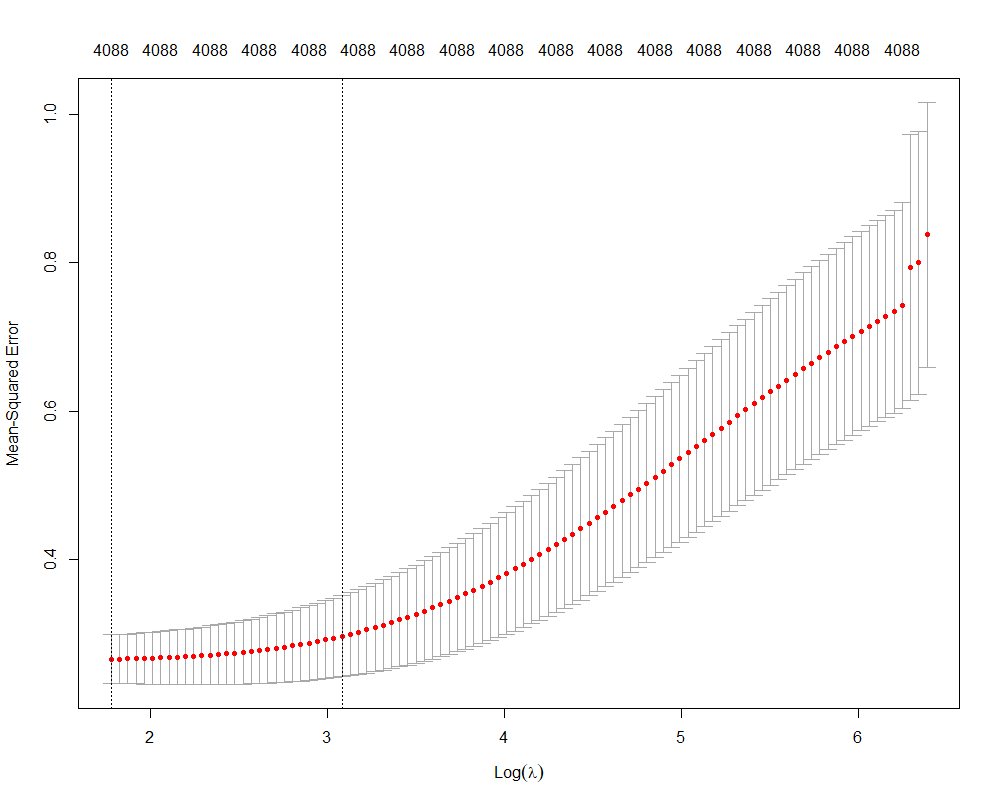
\includegraphics[width=0.45\textwidth]{MS1.png}}
\subfloat[]{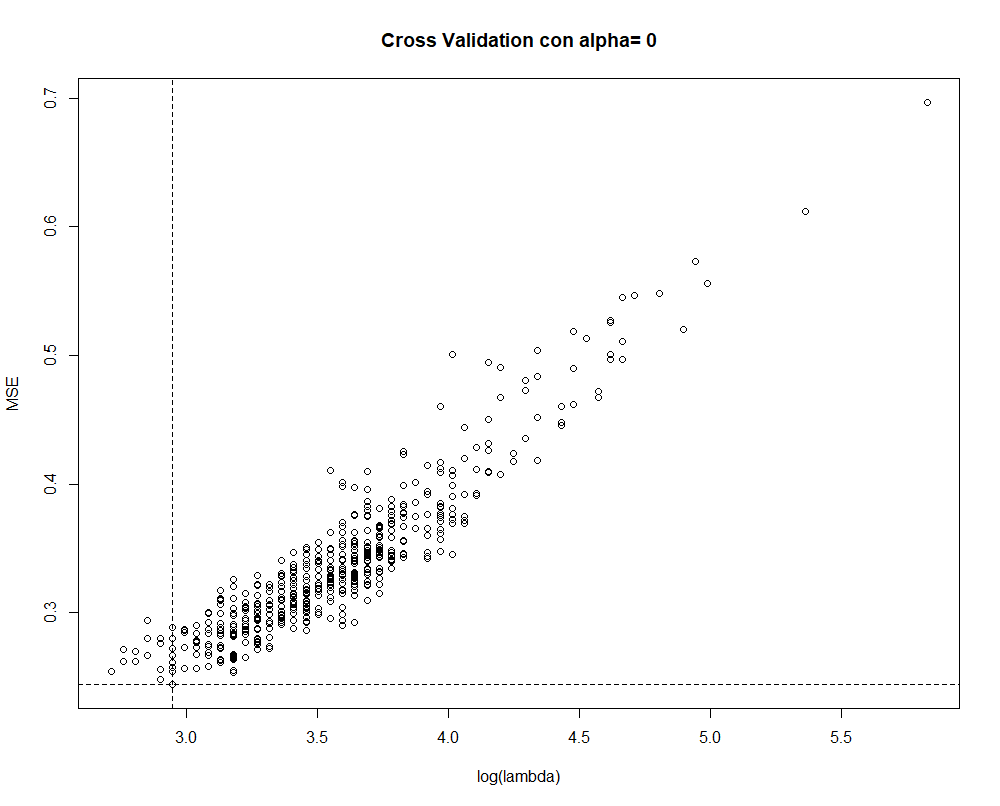
\includegraphics[width=0.45\textwidth]{MSCV1.png}} \hfill \hfill
\subfloat[]{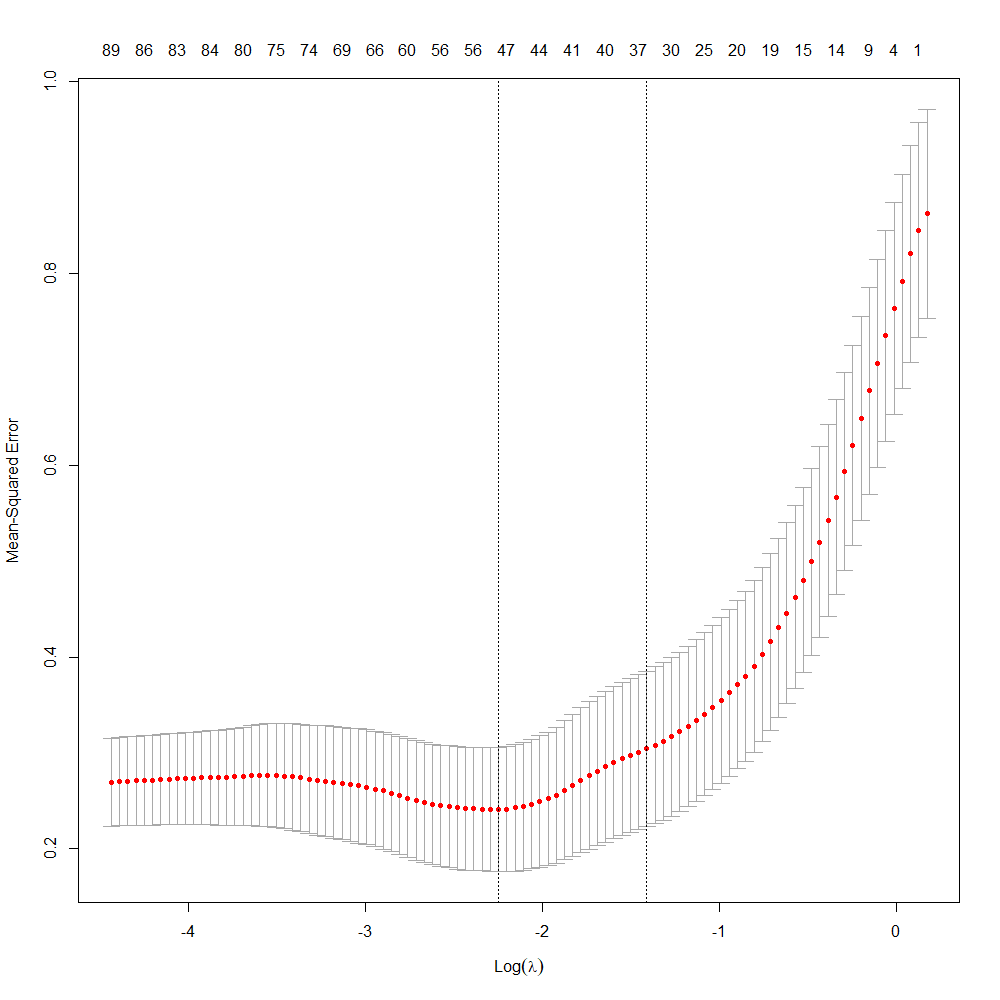
\includegraphics[width=0.45\textwidth]{MS2.png}}
\subfloat[]{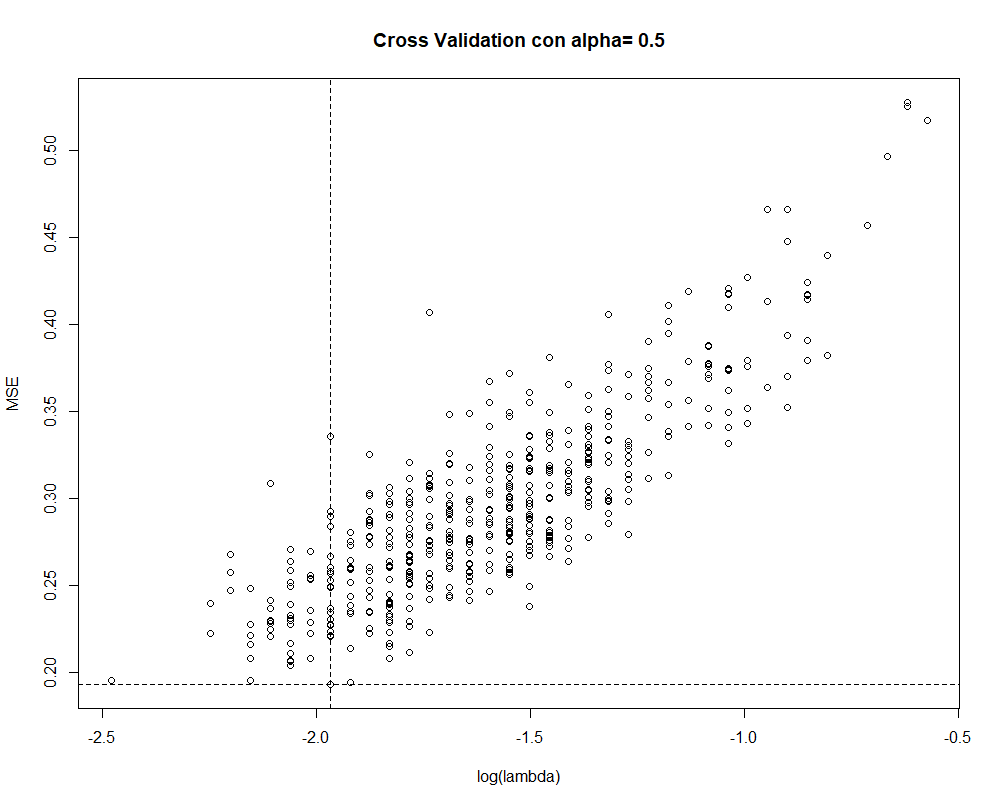
\includegraphics[width=0.45\textwidth]{MSCV2.png}} \hfill
\subfloat[]{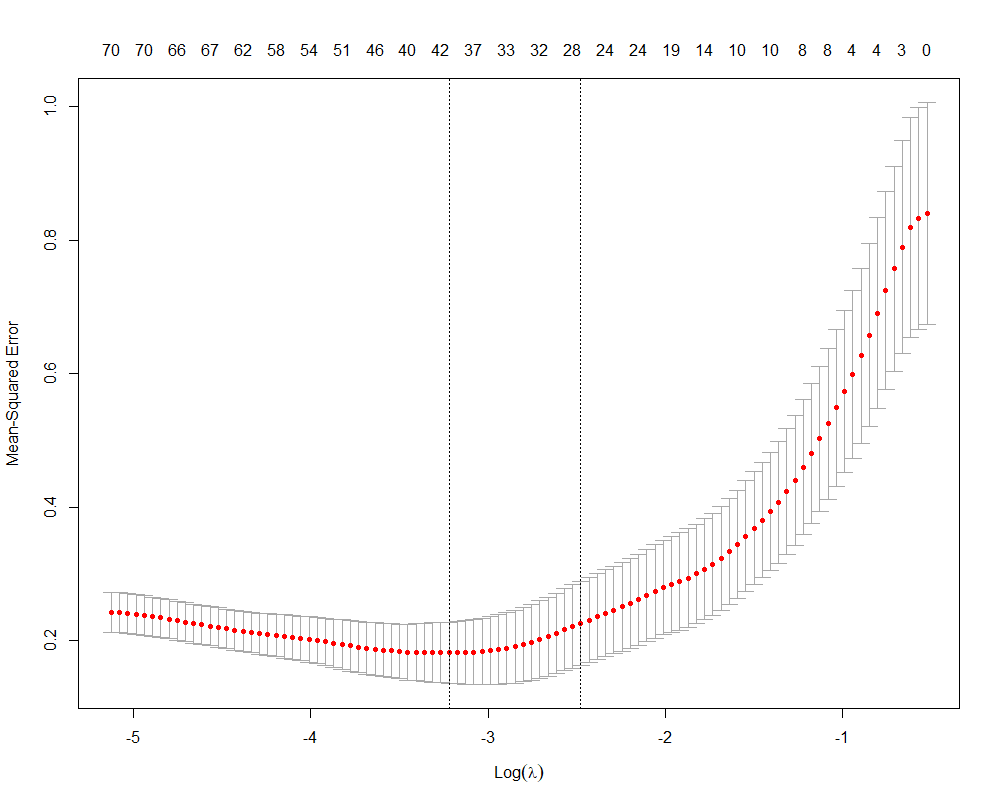
\includegraphics[width=0.45\textwidth]{MS3.png}}
\subfloat[]{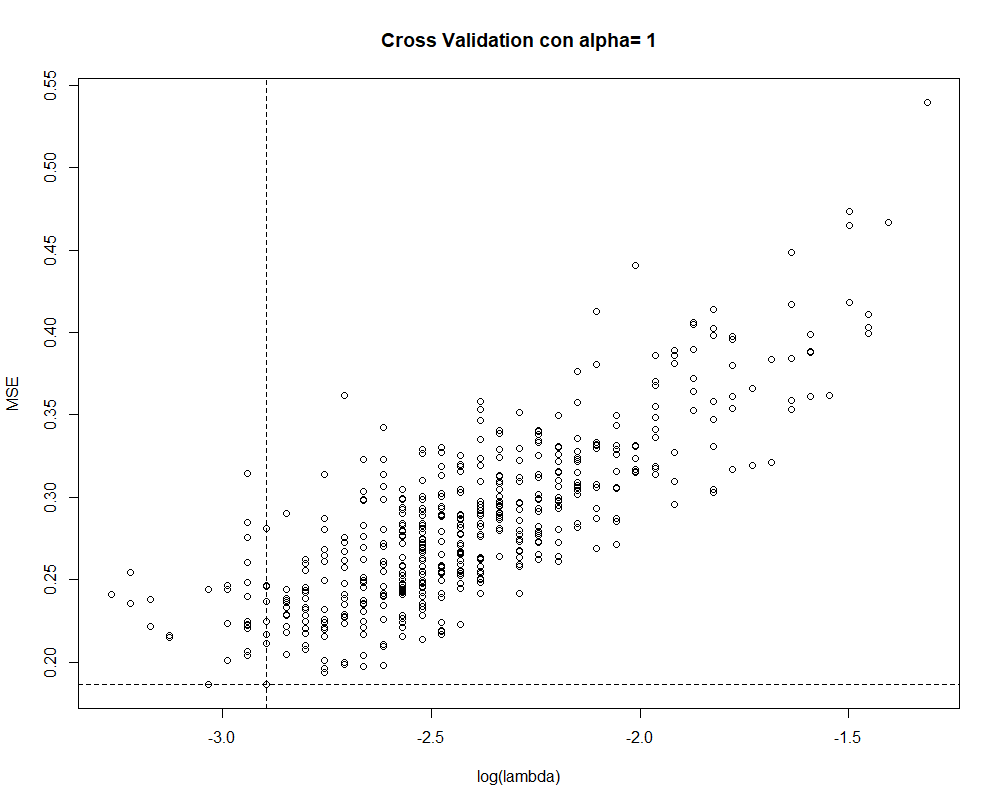
\includegraphics[width=0.45\textwidth]{MSCV3.png}} \hfill
    \caption{Perfiles de errores por Cross validataion para: (a) Ridge con 1 repetición; (b) Ridge con 500 repeticiones; (c) para Elasticnet con 1 repetición, (d) para Ridge con 500 repeticiones, (e) para Lasso con 1 repetición; (f) para Lasso con 500 repeticiones.}\label{fig:MS}
\end{figure}

De la figura \ref{fig:MS} podemos notar que el error que presenta el valor mínimo de $\lambda$ con una repetición a veces resulta ser mayor que el valor de 1se para alguna otra repetición. O bien que para un mismo valor de lambda el error cambia, y este efecto, pensamos, puede deberse a la semilla con la que se realiza el cálculo del error.

%\printbibliography
\end{document}